% !TeX spellcheck = es_ES
%\chapter{Cap\'{\i}tulo 3}
%\chapter{Solution Proposal}
\chapter{Propuesta de solución}
En esta sección se propone una extensión para los EP que apoya el desarrollo de la representación del dominio de la simulación de procesos EOR. Adicionalmente, se conceptualizan los términos derivados de las ecuaciones presentadas en el marco teórico, a partir de los cuales se generan las relaciones estructurales. Posteriormente, se muestra el EP completo de la simulación y se explican por secciones los conceptos principales o clases y los eventos que ejecutan la simulación.

Esta sección se estructura así: en la sección \ref{sec:PSNew} se presenta el elemento adicional para los EP que permite reutilizar una representación en múltiples secciones del EP y la regla para la obtención de código a partir del nuevo elemento. En la sección \ref{sec:Concepts} se revisan los términos de cada ecuación y su traducción a los conceptos presentes en el EP. En la sección \ref{sec:PS_EOR} se muestra el EP completo y se explican las relaciones dinámicas y eventuales por cada concepto principal.

%In this section we propose one element as an extension for Preconceptual Schemas(PS) which aid the understanding of diverse elements in the oil reservoir simulation domain. In addition, we present further description of the concepts stated in the theoretical framework, with their respective representation in the elaborated PS.
%This section is structured as follows: in section  we present the added elements to PS and their usage in our represented domain. In section  we propose the representation of structural and dynamical behavior of each developed concept in the theoretical framework using PS.

%\section{Added elements to Preconceptual Schemas}\label{sec:PSNew}
%\subsection{Analyst defined subroutines}\label{sec:PS_ADS}
%Analyst defined subroutines are analyst defined functions as proposed by (ref Calle) without the return argument. They use global elements and parameters of the subroutine definition. They are defined for re-using dynamical behavior elements which appear more than once in the PS. Names of both subroutines and functions must differ from operators predefined in the PS. Graphic symbol used for subroutines is the same as used for operators and functions. In figure \# we present graphical representation of analyst defined subroutines.

\section{Extensión al Esquema Preconceptual}\label{sec:PSNew}
\subsection{Subrutinas definidas por el analista}\label{sec:PS_ADS}
Las subrutinas definidas por el analista son funciones definidas tal como \cite{JCalle} propuso, pero carecen de un concepto retorno ``return''. Estas utilizan elementos globales y también pueden recibir parámetros adicionales, su representación gráfica es igual a la de una función, pero en su uso no hay una asignación. En la figura \ref{fig:Subroutine} se presenta la representación gráfica y su traducción a código. %\citep{AG01}.
%Nota: Poner tabla y gráfica de uso

%\section{Conceptualization}\label{sec:Concepts}
\section{Conceptualización}\label{sec:Concepts}
En esta sección se traducen las ecuaciones algebraicas, resultantes de la discretización del modelo Black-Oil extendido y las ecuaciones constitutivas usando el método de los volúmenes finitos, a los conceptos principales y su respectiva categoría. 

%\subsection{Mesh}
\subsection{Malla}
Al resolver el dominio espacial continuo como un conjunto discreto de celdas (discretizar el espacio), aparecen propiedades tales como los volúmenes de las celdas y el área de las caras. Este conjunto discreto de celdas es el que denominamos como ``malla''. A su vez, la celda es vista como un conjunto discreto de caras que generan una superficie cerrada\footnote{En el caso tridimensional}. Cada celda cuenta con una numeración, esta sirve para identificar órdenes de solución y ubicación de vecinos para el cálculo del flujo discretizado.

Luego: 
%Poner ecuación acá con Volumen de celda ya como concepto

%\subsection{Rock}
\subsection{Roca}


\subsection{Fluido}
%\subsection{Phase}
%
\subsection{Interacción Interfluido}
%\subsection{Inter-phase interaction}
%
%\subsection{Component}
%
%\subsection{Equlibrium Relation}
\subsection{Relación de Equilibrio}
%
%\subsection{Well}
\subsection{Pozo}

\section{PS Representation of Enhanced Oil Recovery Simulation}\label{sec:PS_EOR}
In this section we propose a PS representation for enhanced oil recovery simulation, we couple a black oil model discretized using finite volumes method with the theoretical framework developed the previous chapter. We mapped each term in the resultant equations to their respective concepts and how they are linked together. The complete representation is shown in \ref{fig:PSComplete}.\\
\begin{figure}[h]
\centering%
\includegraphics[width=0.9\linewidth]{Kap4/MultifasicoSinPozos.pdf}%
\caption{Complete PS Representation for EOR Processes} \label{fig:PSComplete}
\end{figure}

The rest of this section is as follows: In section \ref{sec:PS_Mesh} we present the Mesh concept as a collection of cells with additional elements needed for calculating the attributes of each cell. Furthermore, we develop the dynamical relationship ``Geomodeler defines Mesh'' as an interaction of the role ``Geomodeler'' with atomic\footnote{atomic as is stated by \cite{AG01} (Aca debe ir Zapata)} dynamical relationships. In section \ref{sec:PS_Rock} we present the Rock concept with its attributes and initial characterization. In section \ref{sec:PS_Phase} ... In section \ref{sec:PS_Interphase} ... In section \ref{sec:PS_Equilibrium} we define the partition coefficients as relations between two phases, one contributing mass and another receiving mass in the mass balance equation. In section \ref{sec:PS_Well}  

\subsection{Mesh}\label{sec:PS_Mesh}

We propose a representation of a mesh as a collection of cells which are represented likewise. collection of faces plus their respective attributes. This representation accounts for orthogonal cartesian meshes. Those are generated using the number of cells in each axis or direction, the thickness and top for each cell. Nevertheless, the thickness is only needed for the number of cells defined in every axis, because we work with regular meshes. Therefore the rest of the cells will have the same thickness.
\\
The top of the mesh is required for the first XY plane, and needs to be filled with the depths of each cell in that plane, the rest of the cells are calculated using the depth of the first plane.

The representation stated for Mesh only accounts for orthogonal cartesian meshes, which can be generated with information about number of cells in each axis, their thickness and tops. A (The information above is inserted by a) Geomodeler with defines the mesh by inserting for each axis the number of cells and the thickness for cells in that direction. Once 
\ref{fig:Mesh}.\\
\begin{figure}[h]
	\centering%
	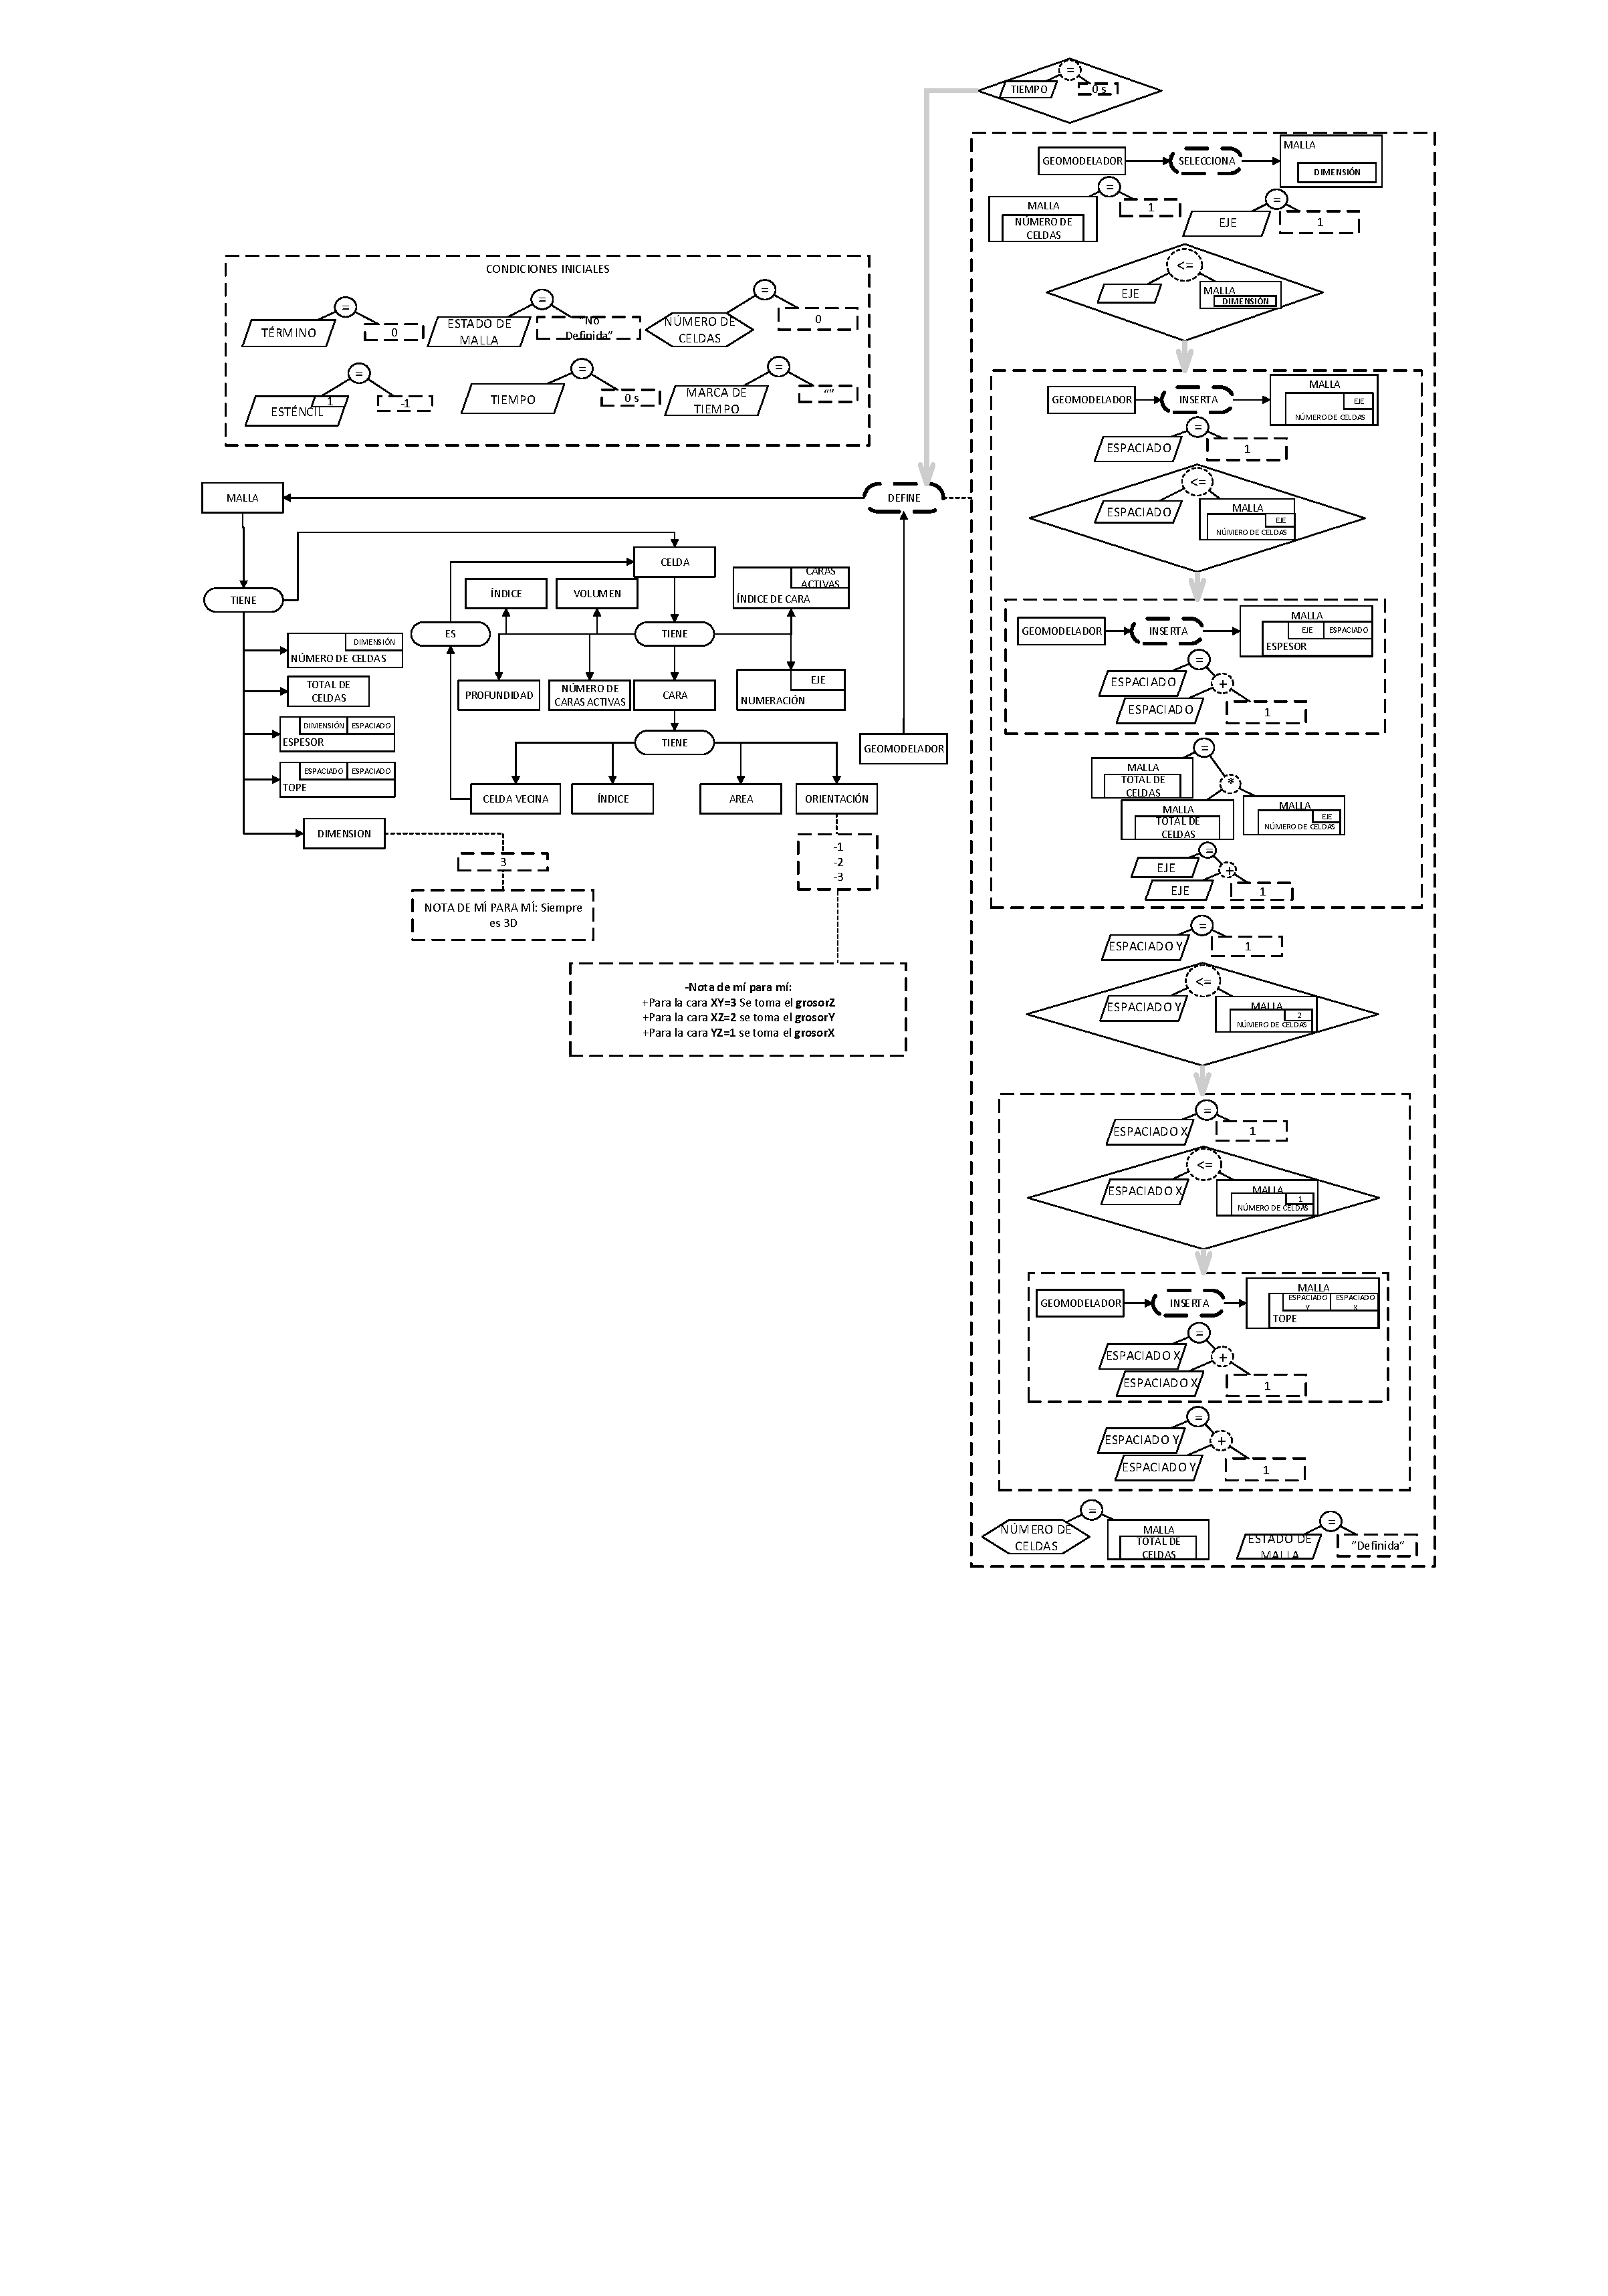
\includegraphics[width=0.9\linewidth]{Kap4/Mesh.pdf}%
	\caption{Mesh definition.} \label{fig:Mesh}
\end{figure}

\subsection{Rock}\label{sec:PS_Rock}
\ref{fig:Rock}.\\
\begin{figure}[h]
	\centering%
	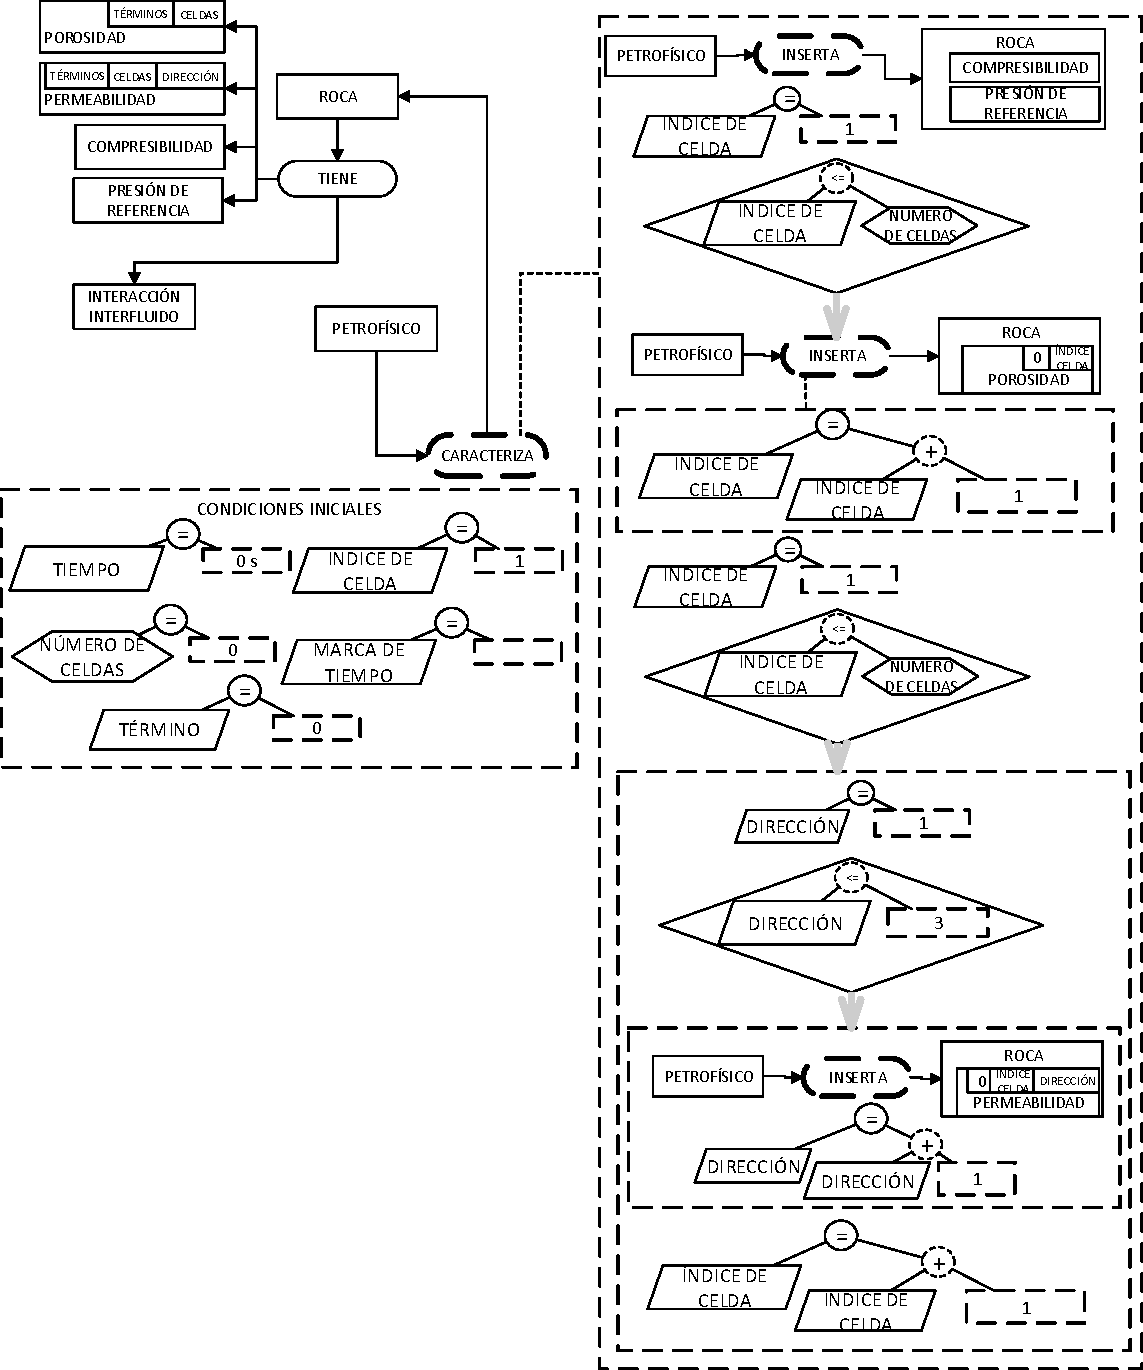
\includegraphics[width=0.9\linewidth]{Kap4/Rock.pdf}%
	\caption{Fluid Characterization.} \label{fig:Rock}
\end{figure}
\subsection{Phase}\label{sec:PS_Phase}

\ref{fig:Fluid}.\\
\begin{figure}[h]
	\centering%
	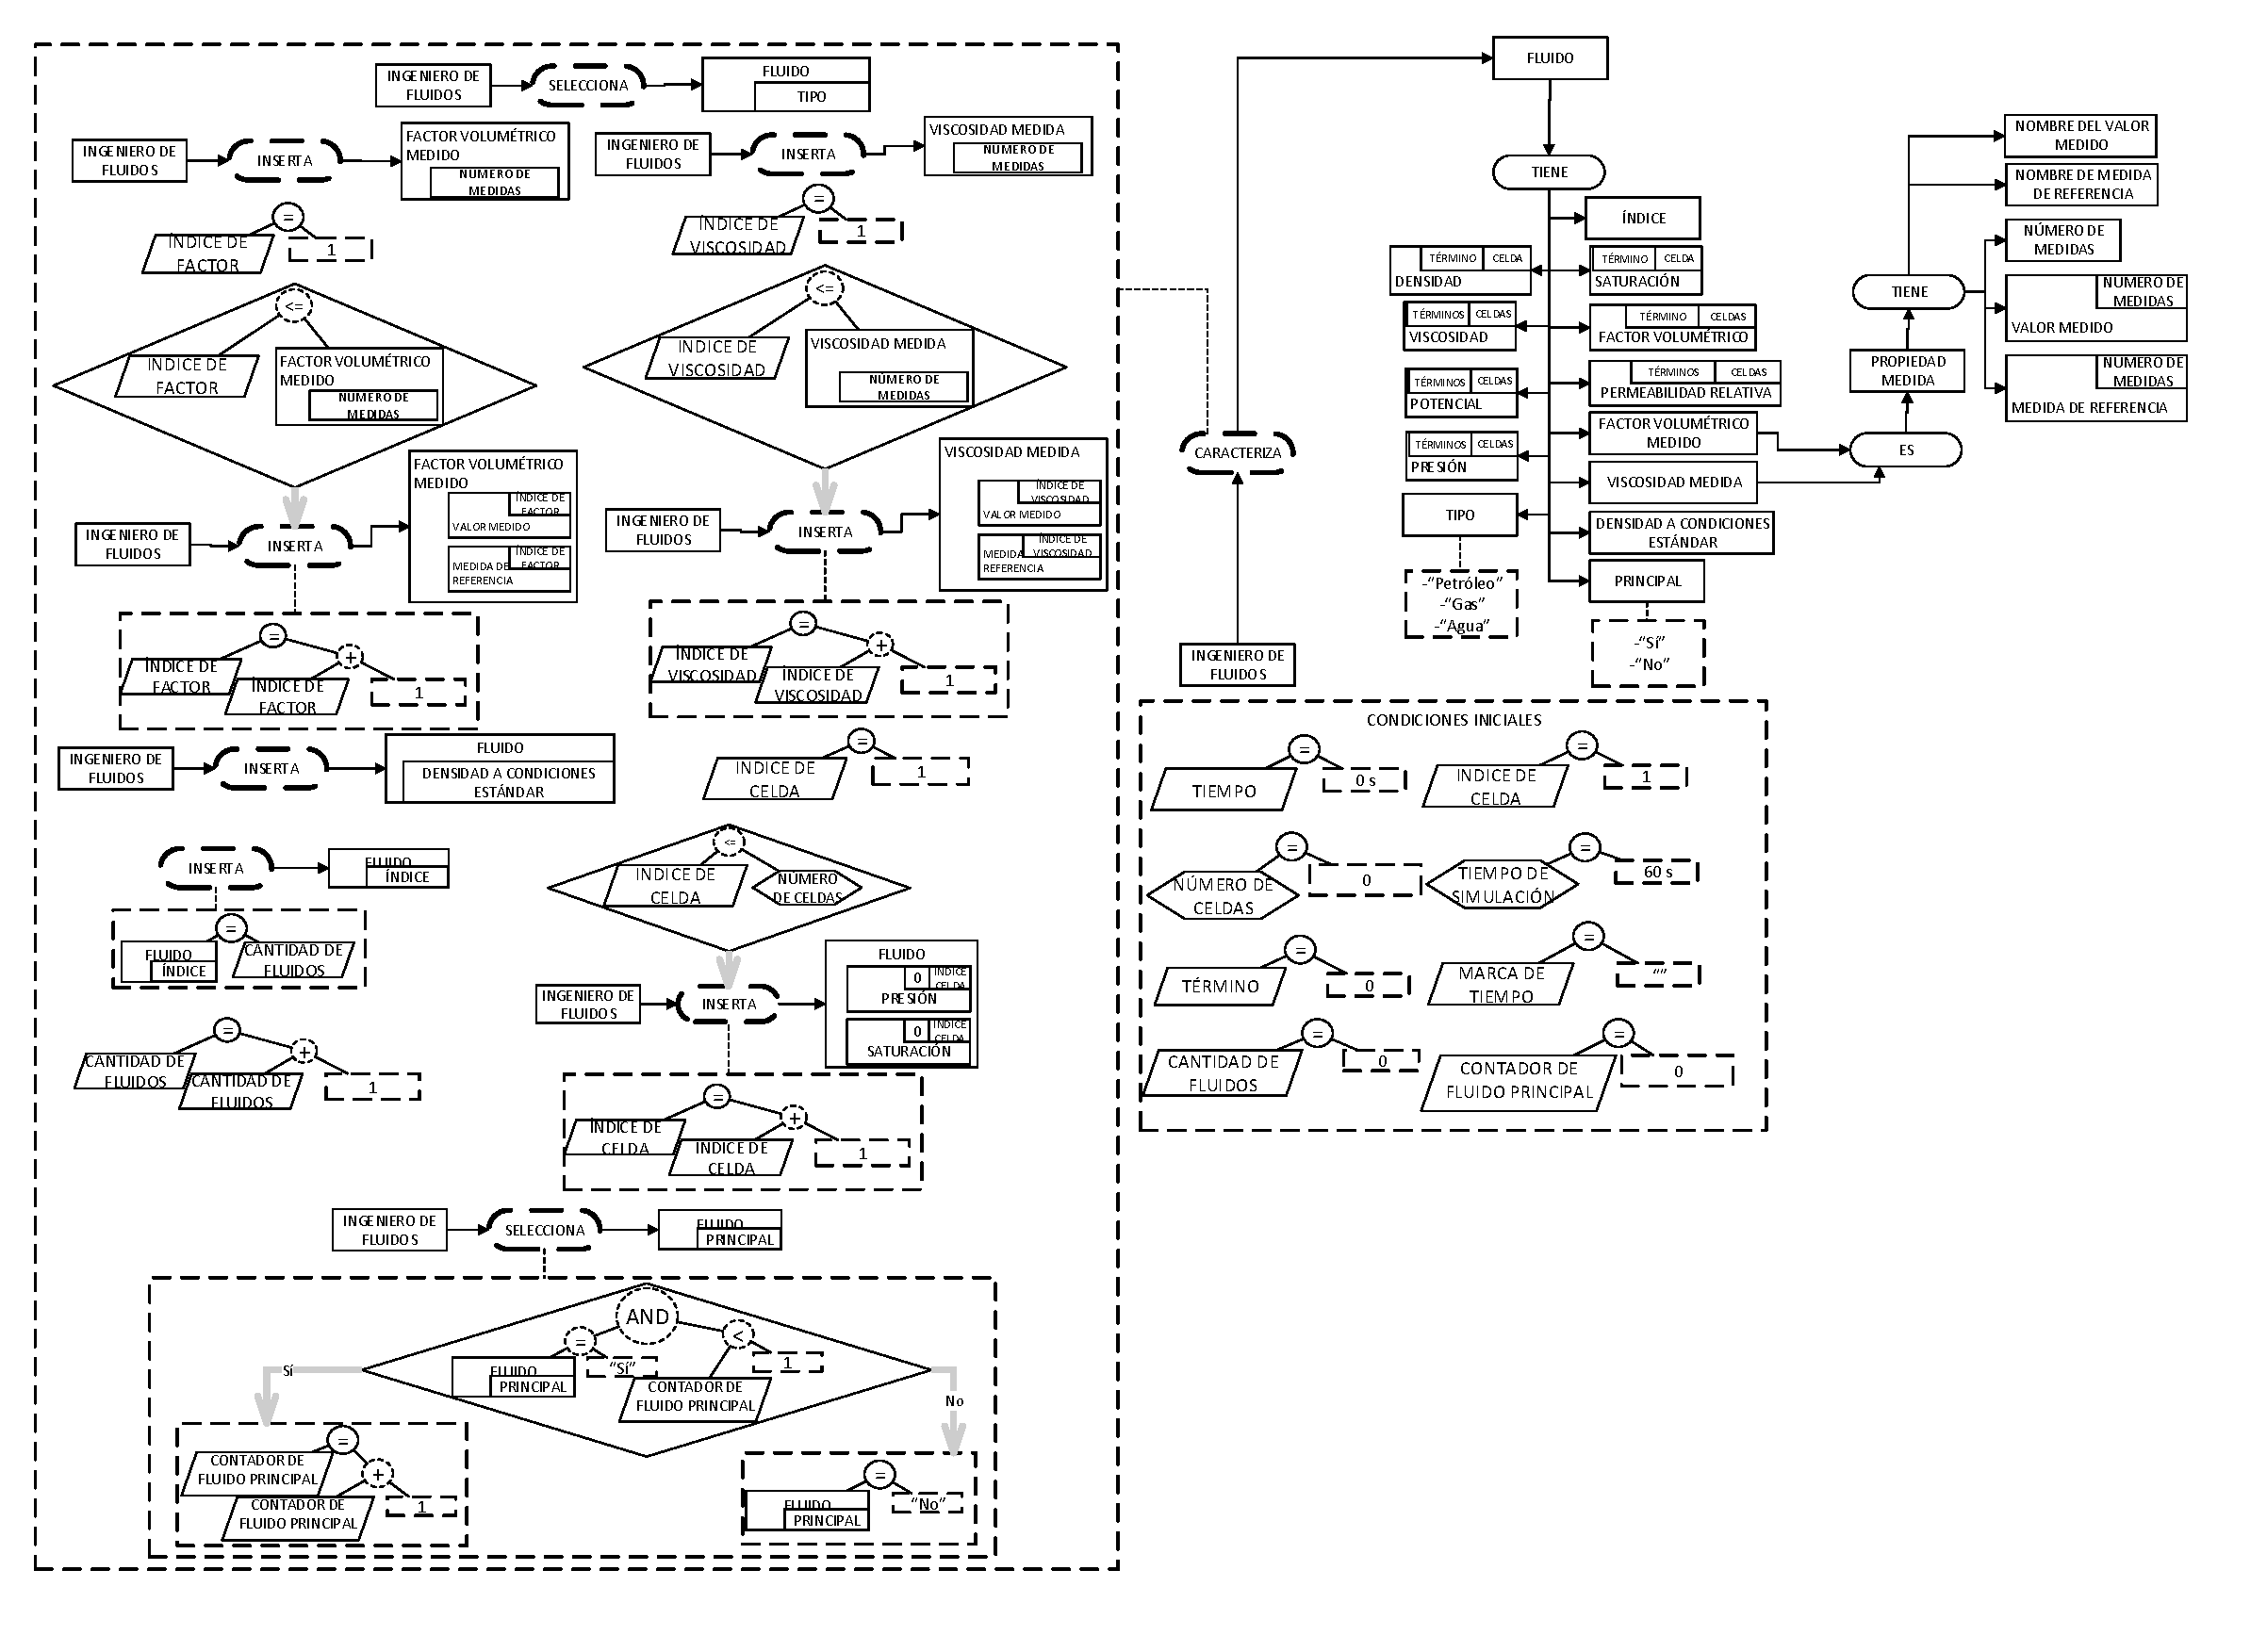
\includegraphics[width=0.9\linewidth]{Kap4/Fluid.pdf}%
	\caption{Fluid Characterization.} \label{fig:Fluid}
\end{figure}

\subsection{Inter-phase interaction}\label{sec:PS_Interphase}

%\subsection{Component}\label{sec:PS_Component} % This could be changed to Chemical

\subsection{Equilibrium Relation}\label{sec:PS_Equilibrium}

\subsection{Well}\label{sec:PS_Well}

%includefigure{Graphical Representation of subroutine}

%includegraphic{Code Translation}

%Se deben incluir tantos cap\'{\i}tulos como se requieran; sin embargo, se recomienda que la tesis  o trabajo de investigaci\'{o}n tenga un m\'{\i}nimo 3 cap\'{\i}tulos y m\'{a}ximo de 6 cap\'{\i}tulos (incluyendo las conclusiones).\\